\section{AI set}

\begin{frame}
	\frametitle{No free lunch}
	
	\begin{itemize}
		\item No general purpose learning algorithm exists \cite{Wolpert96}
		\item Always target functions and training sets with poor performance
	\end{itemize}
	
	\begin{block}{Example}
		\begin{itemize}
			\item Given a classification problem on $\mathbb{N}$ with training set $X=\{1,2\}$ and $Y=\{-1,-1\}$.
			\item How to generalize?
			\item Introducing bias for one class of functions
		\end{itemize}
	\end{block}
\end{frame}

\begin{frame}
	\frametitle{AI set}
	\begin{columns}
		\begin{column}{7.5cm}
			\begin{itemize}
				\item No need for general purpose learning algorithm
				\item Restriction to set of functions involved in intelligent behaviour: \emph{AI-set}
				\item No explicit and implicit specification available
				\item Human brain working proof of feasibility of AI
			\end{itemize}
		\end{column}
		\begin{column}{4cm}
			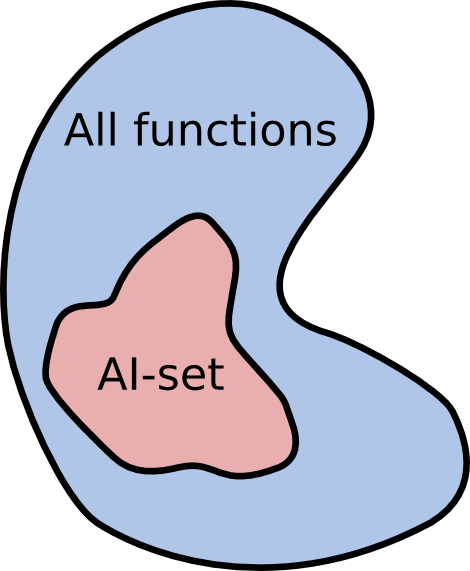
\includegraphics[width=4cm]{images/AIset.png}
		\end{column}
	\end{columns}
\end{frame}

\begin{frame}
	\frametitle{Desiderata for learning algorithms}
	\begin{itemize}
		\item Learn functions of the AI set
	\end{itemize}
	\begin{block}{Quality criteria}
		\begin{enumerate}
			\item Computational efficiency
			\note[item]{Computational complexity during training and recognition}
			\item Statistical efficiency
			\note[item]{Number of data required for good generalization}
			\item Minimal human involvement
			\note[item]{Specification of prior-knowledge, amount of hand-tailoring}
		\end{enumerate}
	\end{block}
\end{frame}

\begin{frame}
	\frametitle{Prior-knowledge}
	\begin{columns}
		\begin{column}{6.5cm}
			\begin{itemize}
				\item Incorporation of prior knowledge
				\begin{enumerate}
					\item Data representation
					\note[item]{Preprocessing, feature extraction}
					\item Machine architecture
					\note[item]{Which functions can the machine represent}
					\item Loss function and regularizer
					\note[item]{How are the functions evaluated and which functions are preferred in the absence of training data}
				\end{enumerate}
				\item Humans learning based on hierarchy of abstractions
				\note[item]{At first we learn basic concepts and then continue to learn higher level concepts based on the former learned abstractions}
				\item Multi-level architecture seems profitable
			\end{itemize}
		\end{column}
		\begin{column}{5cm}
			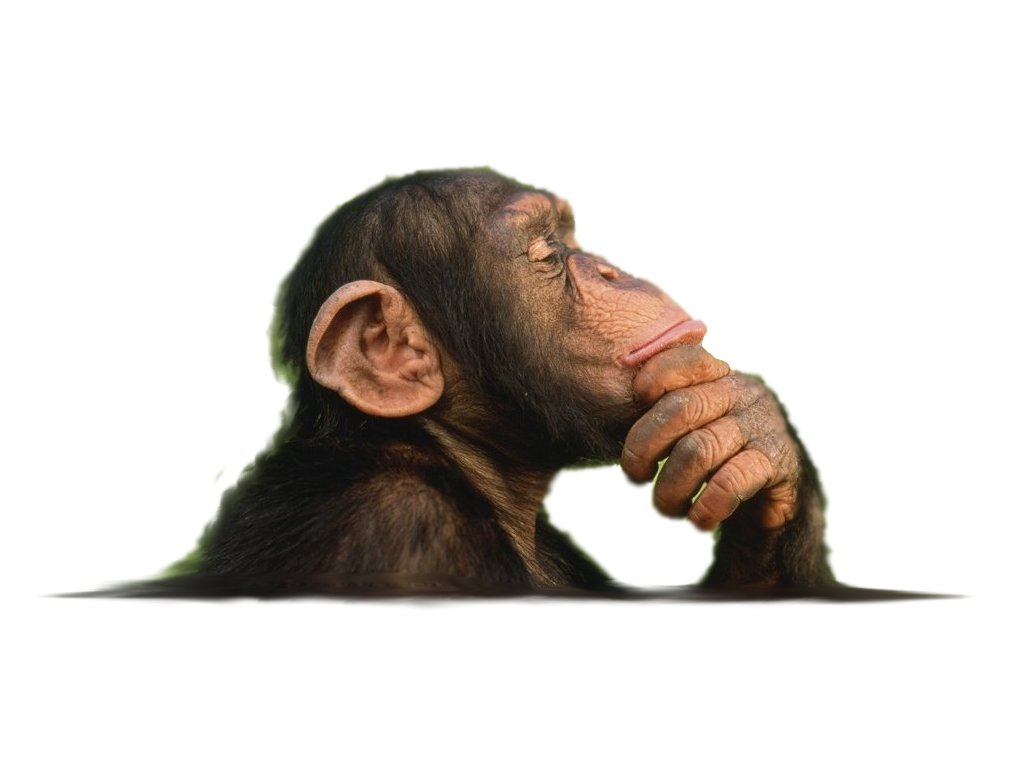
\includegraphics[width=5cm]{images/ape.jpg}
		\end{column}
	\end{columns}
\end{frame}

